\section{Model description}\label{apndx:model}

\textbf{\textit{Atrial Fibrillation.}} The model has four discrete control locations, four state variables, and nonlinear ODEs. A typical set of ODEs in the model is:
\begin{eqnarray*}
\frac{du}{dt} &=& e + (u-\theta_v)(u_u-u ) v g_{fi} + wsg_{si}-g_{so}(u)\\
\frac{ds}{dt} &=& \displaystyle\frac{g_{s2}}{(1+\exp(-2k(u-us)))} -  g_{s2}s\\
\frac{dv}{dt} &=& -g_v^+\cdot v \hspace{1cm} \frac{dw}{dt} = -g_w^+\cdot w
\end{eqnarray*}
The exponential term on the right-hand side of the ODE is the sigmoid function, which often appears in modelling biological switches.

\textbf{\textit{Electronic Oscillator.}}The 3dOsc model represents an electronic oscillator model that contains nonlinear ODEs such as the following.
\begin{eqnarray*}
\frac{dx}{dt} &=& - ax \cdot sin(\omega_1 \cdot \tau)\\
\frac{dy}{dt} &=& - ay \cdot sin( (\omega_1 + c_1) \cdot \tau) \cdot sin(\omega_2)\cdot 2\\
\frac{dz}{dt} &=& - az \cdot sin( (\omega_2 + c_2) \cdot \tau) \cdot cos(\omega_1)\cdot 2\\
\frac{\omega_1}{dt} &=& - c_3\cdot \omega_1\ \ \ \frac{\omega_2}{dt} = -c_4\cdot\omega_2\ \ \ \frac{d\tau}{dt} = 1
\end{eqnarray*}

\textbf{\textit{Quadcopter Control.}} We developed a model that contains the full dynamics of a quadcopter. We use the model to solve control problems by answering reachability questions. A typical set of the differential equations are the following.
\begin{eqnarray*}
\frac{\mathrm{d}\omega_x}{\mathrm{d}t} &=& L\cdot k\cdot (\omega_1^2 - \omega_3^2)(1/I_{xx})-(I_{yy} - I_{zz})\omega_y\omega_z/I_{xx}\\
\frac{\mathrm{d}\omega_y}{\mathrm{d}t} &=& L\cdot k\cdot(\omega_2^2 - \omega_4^2)(1/I_{yy})-(I_{zz} - I_{xx})\omega_x\omega_z/I_{yy}\\
\frac{\mathrm{d}\omega_z}{\mathrm{d}t} &=& b\cdot(\omega_1^2 - \omega_2^2 + \omega_3^2 - \omega_4^2)(1/I_{zz})-(I_{xx} - I_{yy})\omega_x\omega_y/I_{zz}\\
\frac{\mathrm{d}\phi}{\mathrm{d}t} &=& \omega_x + \displaystyle{\frac{\sin\left(\phi\right) \sin\left(\theta\right)}{{\left(\frac{\sin\left(\phi\right)^{2} \cos\left(\theta\right)}{\cos\left(\phi\right)} + \cos\left(\phi\right) \cos\left(\theta\right)\right)} \cos\left(\phi\right)}}\omega_y\\
& &+\displaystyle\frac{\sin\left(\theta\right)}{\frac{\sin\left(\phi\right)^{2} \cos\left(\theta\right)}{\cos\left(\phi\right)} + \cos\left(\phi\right) \cos\left(\theta\right)}\omega_z\\
\frac{\mathrm{d}\theta}{\mathrm{d}t} &=& -(\displaystyle\frac{\sin\left(\phi\right)^{2} \cos\left(\theta\right)}{{\left(\frac{\sin\left(\phi\right)^{2} \cos\left(\theta\right)}{\cos\left(\phi\right)}\omega_y + \cos\left(\phi\right) \cos\left(\theta\right)\right)} \cos\left(\phi\right)^{2}}\\
& &+ \frac{1}{\cos\left(\phi\right)})\omega_y -\displaystyle\frac{\sin\left(\phi\right) \cos\left(\theta\right)}{{\left(\frac{\sin\left(\phi\right)^{2} \cos\left(\theta\right)}{\cos\left(\phi\right)} + \cos\left(\phi\right) \cos\left(\theta\right)\right)} \cos\left(\phi\right)}\omega_z \\
\frac{\mathrm{d}\psi}{\mathrm{d}t} &=& \displaystyle\frac{\sin\left(\phi\right)}{{\left(\frac{\sin\left(\phi\right)^{2} \cos\left(\theta\right)}{\cos\left(\phi\right)} + \cos\left(\phi\right) \cos\left(\theta\right)\right)} \cos\left(\phi\right)}\omega_y\\
& &+ \displaystyle\frac{1}{\frac{\sin\left(\phi\right)^{2} \cos\left(\theta\right)}{\cos\left(\phi\right)} + \cos\left(\phi\right) \cos\left(\theta\right)}\omega_z\\
\frac{\mathrm{d}{xp}}{\mathrm{d}t} &=& (1/m)(\sin(\theta)\sin(\psi)k(\omega_1^2 + \omega_2^2 +\omega_3^2+\omega_4^2) - k\cdot d\cdot{xp})\\
\frac{\mathrm{d}{yp}}{\mathrm{d}t} &=& (1/m)(-\cos(\psi)\sin(\theta)k(\omega_1^2 + \omega_2^2 +\omega_3^2+\omega_4^2) - k\cdot d\cdot{yp})\\
\frac{\mathrm{d}{zp}}{\mathrm{d}t} &=& (1/m)(-g-\cos(\theta)k(\omega_1^2 + \omega_2^2 +\omega_3^2+\omega_4^2) - k\cdot d\cdot{zp}\\
\frac{\mathrm{d}x}{\mathrm{d}t} &=& {xp}, \frac{\mathrm{d}y}{\mathrm{d}t} = {yp}, \frac{\mathrm{d}z}{\mathrm{d}t} = {zp}
\end{eqnarray*}

\textbf{\textit{Prostate Cancer Treatment.}} The Prostate Cancer Treatment model exhibits more nonlinear ODEs. 
\begin{eqnarray*}
\frac{dx}{dt} &=& (\alpha_x
(k_1+(1-k_1)\frac{z}{z+k_2}-\beta_x( (1-k_3)\frac{z}{z+k_4}+k_3))\\
& &- m_1(1-\frac{z}{z_0}))x + c_1 x\\
\frac{dy}{dt} &=& m_1(1-\frac{z}{z_0})x+(\alpha_y (1- d\frac{z}{z_0}) - \beta_y)y+c_2y\\
\frac{dz}{dt} &=& \frac{-z}{\tau} + c_3z\\
\frac{dv}{dt} &=& (\alpha_x
(k_1+(1-k_1)\frac{z}{z+k_2}-\beta_x(k_3+(1-k_3)\frac{z}{z+k_4}))\\
& &- m_1(1-\frac{z}{z_0}))x + c_1 x + m_1(1-\frac{z}{z_0})x+(\alpha_y (1- d\frac{z}{z_0})\\
& &- \beta_y)y+c_2y
\end{eqnarray*}

\begin{figure*}[ht]
\centering
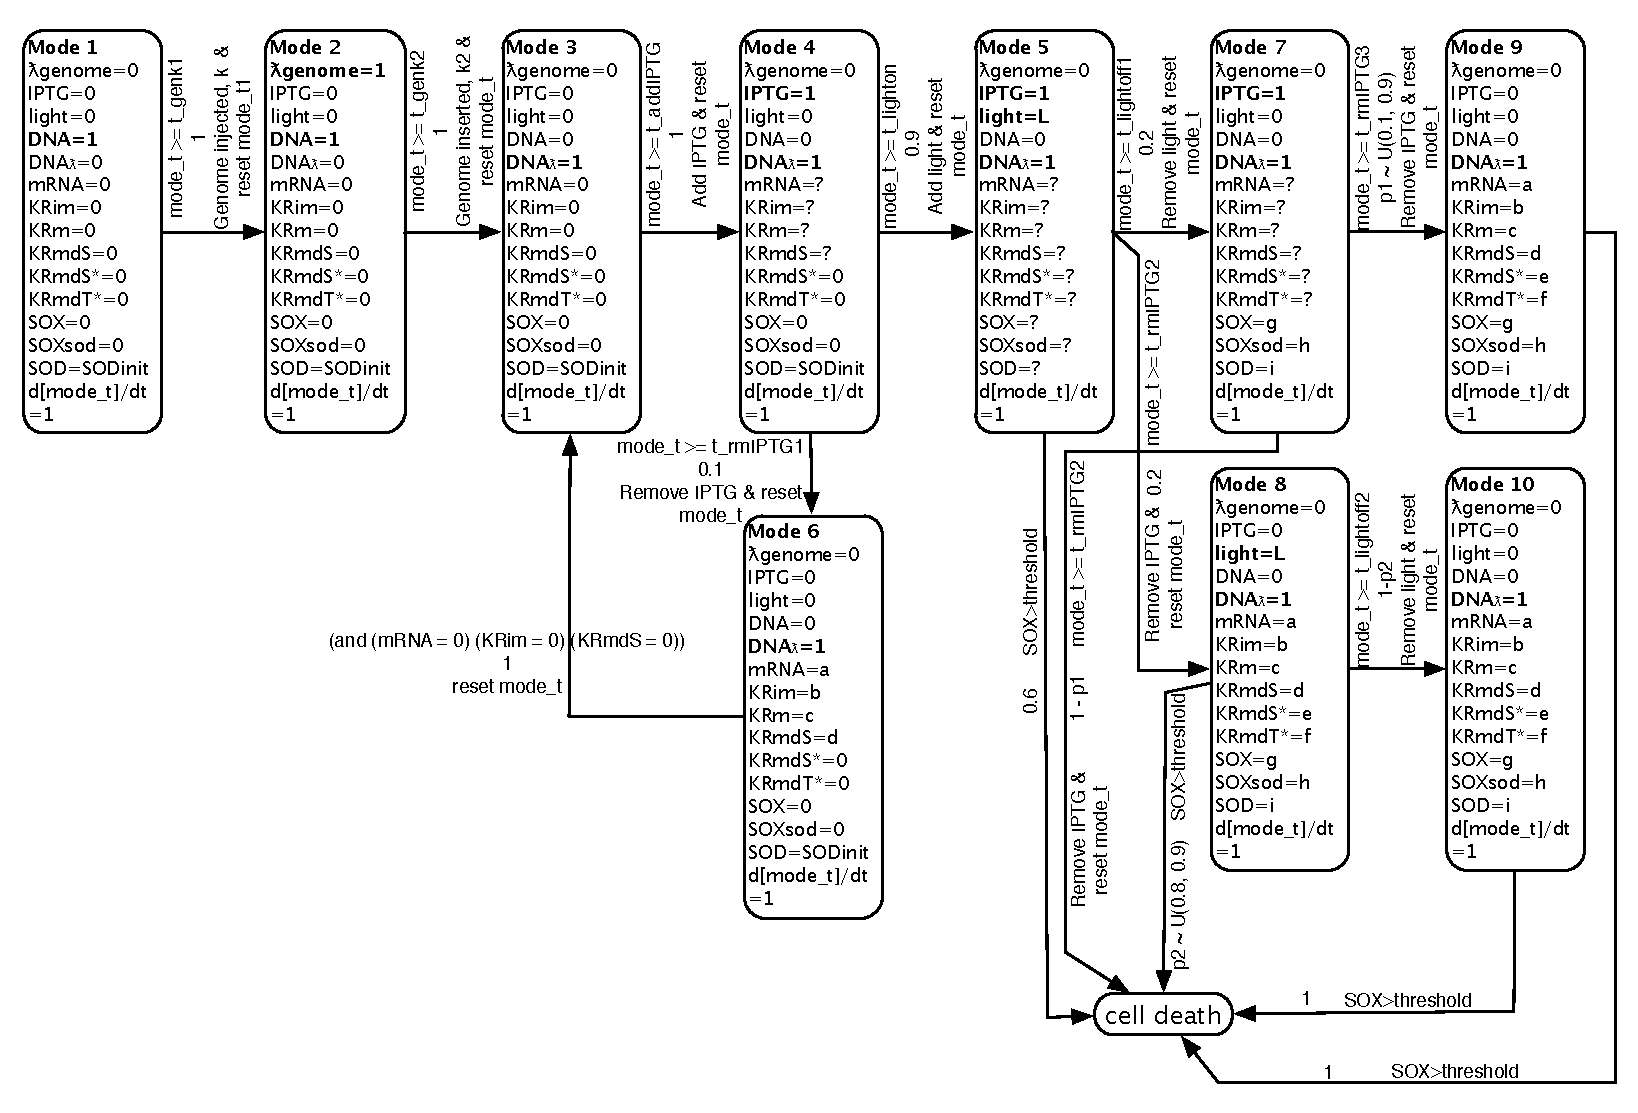
\includegraphics[width=\linewidth]{killerredmodel}
\caption{A probabilistic hybrid automaton for synthesized phage-based therapy model}
\label{fig:killerred}
\end{figure*}

\textbf{\textit{Synthesized Killerred Model.}} The ODEs missing in Figure \ref{fig:killerred} are as follows.
\begin{eqnarray*}
\frac{\mathrm{d}[mRNA]}{\mathrm{d}t} & =& k_{RNAsyn} \cdot [DNA] - k_{RNAdeg} \cdot [mRNA]\\
\frac{\mathrm{d}[KR_{im}]}{\mathrm{d}t} & =& k_{KR_{im}syn} \cdot [mRNA] - (k_{KR_m} + k_{KR_{im}deg})\\
& & \cdot [KR_{im}]\\
\frac{\mathrm{d}[KR_{mdS}]}{\mathrm{d}t} &=& k_{KR_{m}} \cdot [KR_{im}] - k_{KR_{mdS}deg} \cdot [KR_{mdS}]\\
& &(before\; turning \; on \; the \; light)\\
\frac{\mathrm{d}[KR_{mdS}]}{\mathrm{d}t} &=& k_{KR_{m}} \cdot [KR_{im}] + k_{KR_f} \cdot [KR_{mdS^*}] \\
& &+ k_{KR_{ic}} \cdot [KR_{mdS^*}] + k_{KR_{nrd}} \cdot [KR_{mdT^*}]\\
& &+ k_{KR_{SOXd1}} \cdot [KR_{mdT^* }] - k_{KR_{ex}} \cdot [KR_{mdS}]\\
& &- k_{KR_{mdS}deg} \cdot [KR_{mdS}]\;\;\; (after\; adding\; light)\\
\frac{\mathrm{d}[KR_{mdS^*}]}{\mathrm{d}t} &=& k_{KR_{ex}} \cdot [KR_{mdS}] - k_{KR_f } \cdot [KR_{mdS^*}] \\
& &-k_{KR_{ic}} \cdot [KR_{mdS^*}] - k_{KR_{isc}} \cdot [KR_{mdS^*}]\\
& &- k_{KR_{mdS^*}deg} \cdot [KR_{mdS^*}]\\
\frac{\mathrm{d}[KR_{mdT^*}]}{\mathrm{d}t} &=& k_{KR_{isc}} \cdot [KR_{mdS^*}] - k_{KR_{nrd}} \cdot [KR_{mdT^*}]\\
& &- k_{KR_{SOXd1}} \cdot [KR_{mdT^*}]\\
& &- k_{KR_{SOXd2}} \cdot [KR_{mdT^*}]\\
& &- k_{KR_{mdT^*}deg} \cdot [KR_{mdT^*}]
\end{eqnarray*}
\begin{eqnarray*}
\frac{\mathrm{d}[SOX]}{\mathrm{d}t} &=& k_{KR_{SOXd1}} \cdot [KR_{mdT^*}] + k_{KR_{SOXd2}} \cdot [KR_{mdT^*}]\\
& &- \frac{\mathrm{d}[SOX_{sod}]}{\mathrm{d}t}\\
\frac{\mathrm{d}[SOX_{sod}]}{\mathrm{d}t} &=& k_{SOD} \cdot V_{maxSOD} \cdot \frac{[SOX]}{K_m + [SOX]}
\end{eqnarray*}












